\definecolor{fcblue}{HTML}{2A78D6}
\definecolor{fcorange}{HTML}{EB6834}
\definecolor{fcgreen}{HTML}{1BAF7A}
\definecolor{fcgold}{HTML}{EDA100}
\definecolor{fcpink}{HTML}{E87BA4}
\definecolor{fcdgreen}{HTML}{008300}
\definecolor{fcpurple}{HTML}{4A3AA7}
\definecolor{fcred}{HTML}{E34948}
\definecolor{fcgrey}{HTML}{777777}
\pgfplotsset{compat=1.16, fig/.style={tick label style={font=\scriptsize}, label style={font=\scriptsize},
  title style={font=\scriptsize}, every axis plot/.append style={}, grid=major, grid style={draw=black!10, line width=0.3pt},
  axis line style={draw=black!50}, tick style={draw=black!50}, legend style={font=\tiny, draw=none, fill=none}}}
\begin{center}
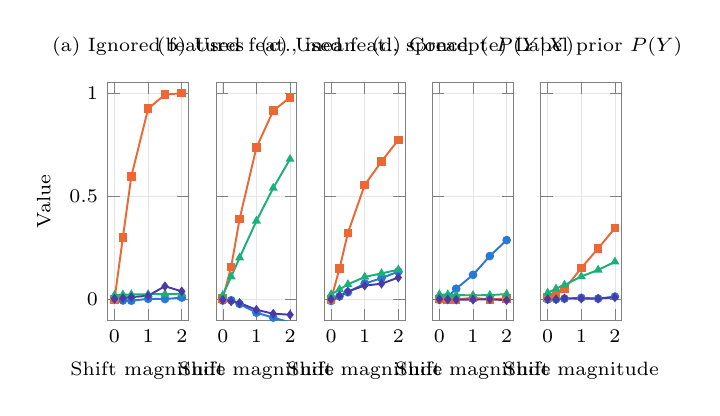
\begin{tikzpicture}
\begin{axis}[name=s0, fig, width=0.215\textwidth, height=4.6cm, ymin=-0.1, ymax=1.05, title={(a) Ignored features}, xlabel={Shift magnitude}, ylabel={Value}, legend to name=syleg, legend columns=4]
\addplot[color=fcblue, mark=*, mark size=1.2pt, line width=0.7pt] coordinates {(0.000,-0.001) (0.250,-0.004) (0.500,-0.005) (1.000,0.004) (1.500,0.003) (2.000,0.010)};
\addlegendentry{Accuracy drop $\Delta$}
\addplot[color=fcorange, mark=square*, mark size=1.2pt, line width=0.7pt] coordinates {(0.000,0.000) (0.250,0.302) (0.500,0.596) (1.000,0.924) (1.500,0.992) (2.000,0.999)};
\addlegendentry{Domain-clf. AUC (rescaled)}
\addplot[color=fcgreen, mark=triangle*, mark size=1.2pt, line width=0.7pt] coordinates {(0.000,0.022) (0.250,0.024) (0.500,0.025) (1.000,0.026) (1.500,0.027) (2.000,0.029)};
\addlegendentry{IWS-KS (ours)}
\addplot[color=fcpurple, mark=diamond*, mark size=1.2pt, line width=0.7pt] coordinates {(0.000,0.004) (0.250,0.007) (0.500,0.012) (1.000,0.019) (1.500,0.065) (2.000,0.040)};
\addlegendentry{Importance-wtd. drop}
\end{axis}
\begin{axis}[name=s1, fig, width=0.215\textwidth, height=4.6cm, ymin=-0.1, ymax=1.05, title={(b) Used feat., mean}, xlabel={Shift magnitude}, at={(s0.east)}, anchor=west, xshift=0.35cm, yticklabels={}]
\addplot[color=fcblue, mark=*, mark size=1.2pt, line width=0.7pt] coordinates {(0.000,-0.004) (0.250,-0.003) (0.500,-0.021) (1.000,-0.063) (1.500,-0.087) (2.000,-0.110)};
\addplot[color=fcorange, mark=square*, mark size=1.2pt, line width=0.7pt] coordinates {(0.000,0.007) (0.250,0.159) (0.500,0.391) (1.000,0.736) (1.500,0.914) (2.000,0.979)};
\addplot[color=fcgreen, mark=triangle*, mark size=1.2pt, line width=0.7pt] coordinates {(0.000,0.021) (0.250,0.111) (0.500,0.203) (1.000,0.381) (1.500,0.540) (2.000,0.680)};
\addplot[color=fcpurple, mark=diamond*, mark size=1.2pt, line width=0.7pt] coordinates {(0.000,-0.001) (0.250,-0.008) (0.500,-0.016) (1.000,-0.049) (1.500,-0.068) (2.000,-0.073)};
\end{axis}
\begin{axis}[name=s2, fig, width=0.215\textwidth, height=4.6cm, ymin=-0.1, ymax=1.05, title={(c) Used feat., spread}, xlabel={Shift magnitude}, at={(s1.east)}, anchor=west, xshift=0.35cm, yticklabels={}]
\addplot[color=fcblue, mark=*, mark size=1.2pt, line width=0.7pt] coordinates {(0.000,-0.006) (0.250,0.016) (0.500,0.036) (1.000,0.078) (1.500,0.104) (2.000,0.136)};
\addplot[color=fcorange, mark=square*, mark size=1.2pt, line width=0.7pt] coordinates {(0.000,0.002) (0.250,0.150) (0.500,0.323) (1.000,0.555) (1.500,0.669) (2.000,0.773)};
\addplot[color=fcgreen, mark=triangle*, mark size=1.2pt, line width=0.7pt] coordinates {(0.000,0.025) (0.250,0.049) (0.500,0.074) (1.000,0.110) (1.500,0.127) (2.000,0.145)};
\addplot[color=fcpurple, mark=diamond*, mark size=1.2pt, line width=0.7pt] coordinates {(0.000,0.002) (0.250,0.018) (0.500,0.040) (1.000,0.068) (1.500,0.077) (2.000,0.107)};
\end{axis}
\begin{axis}[name=s3, fig, width=0.215\textwidth, height=4.6cm, ymin=-0.1, ymax=1.05, title={(d) Concept $P(Y|X)$}, xlabel={Shift magnitude}, at={(s2.east)}, anchor=west, xshift=0.35cm, yticklabels={}]
\addplot[color=fcblue, mark=*, mark size=1.2pt, line width=0.7pt] coordinates {(0.000,-0.001) (0.250,0.013) (0.500,0.053) (1.000,0.120) (1.500,0.211) (2.000,0.288)};
\addplot[color=fcorange, mark=square*, mark size=1.2pt, line width=0.7pt] coordinates {(0.000,0.003) (0.250,0.001) (0.500,0.001) (1.000,0.009) (1.500,0.001) (2.000,0.005)};
\addplot[color=fcgreen, mark=triangle*, mark size=1.2pt, line width=0.7pt] coordinates {(0.000,0.025) (0.250,0.025) (0.500,0.022) (1.000,0.021) (1.500,0.022) (2.000,0.027)};
\addplot[color=fcpurple, mark=diamond*, mark size=1.2pt, line width=0.7pt] coordinates {(0.000,0.003) (0.250,0.001) (0.500,0.000) (1.000,0.000) (1.500,0.002) (2.000,-0.003)};
\end{axis}
\begin{axis}[name=s4, fig, width=0.215\textwidth, height=4.6cm, ymin=-0.1, ymax=1.05, title={(e) Label prior $P(Y)$}, xlabel={Shift magnitude}, at={(s3.east)}, anchor=west, xshift=0.35cm, yticklabels={}]
\addplot[color=fcblue, mark=*, mark size=1.2pt, line width=0.7pt] coordinates {(0.000,0.001) (0.250,0.002) (0.500,0.005) (1.000,0.009) (1.500,0.005) (2.000,0.015)};
\addplot[color=fcorange, mark=square*, mark size=1.2pt, line width=0.7pt] coordinates {(0.000,0.011) (0.250,0.022) (0.500,0.051) (1.000,0.153) (1.500,0.248) (2.000,0.346)};
\addplot[color=fcgreen, mark=triangle*, mark size=1.2pt, line width=0.7pt] coordinates {(0.000,0.033) (0.250,0.053) (0.500,0.071) (1.000,0.112) (1.500,0.144) (2.000,0.183)};
\addplot[color=fcpurple, mark=diamond*, mark size=1.2pt, line width=0.7pt] coordinates {(0.000,0.003) (0.250,0.002) (0.500,0.006) (1.000,0.005) (1.500,0.005) (2.000,0.011)};
\end{axis}
\end{tikzpicture}\\[2pt]
\ref{syleg}
\end{center}
